% Fig. 2.15 / spec Fig A15 -- the p-quantile cuts the distribution into a
%   front part of size p and a back part of size 1-p.
% Source: mathstatch2.tex lines 2439-2478.
%
% Deviations from CH2_FIGURE_SPECS.md:
%
% 1. Curve.  The manuscript uses (45/4) x^3 e^{-1.7x} - 0.15, which does not
%    integrate to 1; per spec 1.6 the web uses Gamma(shape 4, rate 1.7),
%    f(x) = 1.3920167 x^3 e^{-1.7x}, plotted over 0:6.4 at y = 7.6cm.
%
% 2. Boundary.  The manuscript draws it at 1.3, which for this density is the
%    0.117 quantile.  Spec 3.2 item 3 moves it to p = 0.25 but gives the
%    quartile as 1.578, which is wrong: F(1.578) = 0.282075.  Ruling 19
%    settles the value at 1.491365, where f = 0.365865, and that is what is
%    drawn here -- the same number as q_1 of the four-way split in
%    quartiles-equal-areas.tex, so the two adjacent figures agree.  The
%    caption has to say that p = 0.25 here.
%
% 3. Notation of the boundary.  Spec A15 labels it q, following the
%    manuscript, where the same letter q stands both for the value of the
%    quantile and for the number of parts the distribution is cut into.
%    Ruling 18 removes that ambiguity: the value of the p-quantile is written
%    x_p and q is left to mean the number of parts.  The label here is
%    therefore x_p, matching the body text of P212.  Fig. 2.16 keeps q_1, q_2,
%    q_3 per ruling 20; there q really does mean the number of parts, so no
%    ambiguity arises.
%
% 4. Shading path.  The manuscript's \fill starts at (2.6,0), unrelated to the
%    boundary, leaving a notch on the left edge (spec 3.2 item 4).  The path
%    here follows spec 1.6.
%
% 5. Type size of the p and 1-p labels.  The manuscript sets them \small; they
%    are set at \normalsize instead so that nothing in the picture falls below
%    the 12px floor of spec 1.3 on a 350px phone.
%
% 6. The manuscript puts the x label at (6.5,0.15) while the axis stops at
%    6.2.  Per spec 1.3 the label goes at the end of the axis instead.
%
% 7. \DeclareMathSizes{10}{10}{9}{8}, as in the rest of this group; not the
%    site-wide \sssig change that ruling 21 defers.  Native size
%    206.796 x 110.284 pt, drawing range 7.15cm wide, inside the 9.0cm cap; the
%    box is shared with median-intuition.tex and quartiles-equal-areas.tex.
%    At the 350px phone width that gives 16.9px for 10pt text, 15.2px for 9pt
%    scripts and 13.5px for 8pt scriptscripts; at 620px 29.9 / 26.9 / 23.9px.
%
% The density is written as 1.3920167 (x e^{-0.56666667x})^3 because pgfmath
% cannot hold e^{1.7x} at the right hand end of the range.
\documentclass[tikz,border=2pt]{standalone}
\usepackage{amsmath}
\usepackage{amssymb}
\usepackage{xcolor}
\usetikzlibrary{arrows.meta}
\newcommand{\sssig}{\scriptscriptstyle}
\DeclareMathSizes{10}{10}{9}{8}

\definecolor{journalink}{HTML}{1F1C18}
\definecolor{journalmuted}{HTML}{8A7F72}
\definecolor{journalaccent}{HTML}{9C2D2D}

\begin{document}
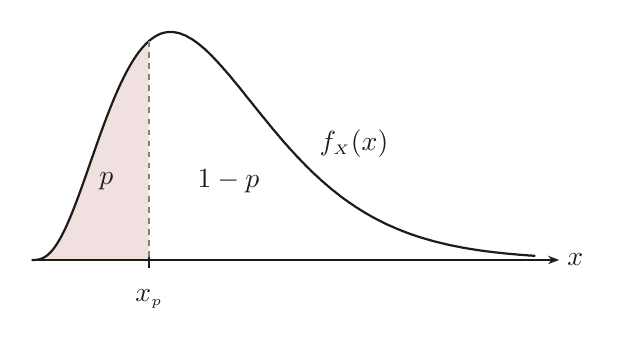
\begin{tikzpicture}[
  x=1cm,
  y=7.6cm,
  every node/.style={font=\normalsize, journalink},
  axis/.style={journalink, line width=0.8pt, -{Stealth[length=4pt]}},
  tick/.style={journalink, line width=0.8pt},
  curve/.style={journalink, line width=0.8pt},
  guide/.style={journalmuted, line width=0.5pt, dash pattern=on 2pt off 2pt},
  region/.style={journalaccent, fill opacity=0.15}
]
  % ---- bounding box shared with the other two Gamma(4,1.7) figures ------
  \path (-0.05cm,-0.80cm) rectangle (7.10cm,2.95cm);

  % ---- the front part, of size p = 0.25 --------------------------------
  \fill[region]
    (0,0) -- (1.491365,0) -- (1.491365,0.365865)
    -- plot[domain=1.491365:0, samples=200, smooth]
       (\x,{1.3920167*pow(\x*exp(-0.56666667*\x),3)}) -- cycle;

  % ---- density curve: Gamma(4, 1.7) ------------------------------------
  \draw[curve] plot[domain=0:6.4, samples=300, smooth]
    (\x,{1.3920167*pow(\x*exp(-0.56666667*\x),3)});

  % ---- x axis ----------------------------------------------------------
  \draw[axis] (0,0) -- (6.7,0);
  \node[anchor=west, inner sep=2.8pt] at (6.7,0) {$x$};

  % ---- the p-quantile --------------------------------------------------
  \draw[guide] (1.491365,0.365865) -- (1.491365,0);
  \draw[tick] ([yshift=0.035cm]1.491365,0) -- ([yshift=-0.106cm]1.491365,0);
  \node[anchor=north] at ([yshift=-0.25cm]1.491365,0) {$x_{\sssig p}$};

  % ---- the two parts ---------------------------------------------------
  \node[inner sep=0pt] at ([yshift=1.00cm]0.950,0) {$p$};
  \node[inner sep=0pt] at ([yshift=1.00cm]2.500,0) {$1-p$};

  % ---- curve label -----------------------------------------------------
  \node[anchor=south west, inner sep=0pt] at ([yshift=1.30cm]3.65,0)
    {$f_{\sssig X}(x)$};
\end{tikzpicture}
\end{document}
